% Intended LaTeX compiler: xelatex
\documentclass[a4paper, 12pt]{article}
\usepackage{graphicx}
\usepackage{longtable}
\usepackage{wrapfig}
\usepackage{rotating}
\usepackage[normalem]{ulem}
\usepackage{amsmath}
\usepackage{amssymb}
\usepackage{capt-of}
\usepackage{hyperref}
\usepackage[danish]{babel}
\usepackage{mathtools}
\usepackage{enumitem}
\usepackage[margin=2.3cm]{geometry}
\hypersetup{colorlinks, linkcolor=black, urlcolor=blue}
\setlength{\parindent}{0em}
\parskip 1.5ex
\author{Jacob Debel}
\date{Fysik B}
\title{Elektriske eksperimenter\\\medskip
\large Elektricitet}
\hypersetup{
 pdfauthor={Jacob Debel},
 pdftitle={Elektriske eksperimenter},
 pdfkeywords={},
 pdfsubject={},
 pdfcreator={Emacs 29.4 (Org mode 9.6.15)}, 
 pdflang={Danish}}
\begin{document}

\maketitle

\section*{Indledning}
\label{sec:org8655e6f}
I skal arbejde med 3 forskellige eksperimenter. Der skal udarbejdes en samet rapport med et fælles teoriafsnit omkring elektricitet, men hvor resten af rapporten er delt mellem de 3 eksperimenter. Slut af med en samlet konklusion.

\tableofcontents

\newpage


\section{En sammenkobling af pærer}
\label{sec:orga16d5f9}

På figur \ref{forsoeg_1} ses en sammenkobling af en spændingskilde og 4 ens pærer. Spændingskilden er repræsenteret ved \(\mathcal{E}\) mens pærerne er repræsenteret ved \(R_1\), \(R_2\), \(R_3\) og \(R_4\).

\begin{figure}[htbp]
\centering
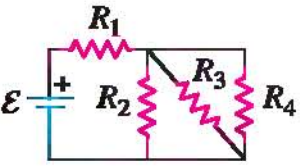
\includegraphics[width=0.4\linewidth]{./img/forsoeg_1.png}
\caption{\label{forsoeg_1}\(\mathcal{E}\) repræsenterer en spændingskilde, mens \(R_1\), \(R_2\), \(R_3\) og \(R_4\) repræsenterer 4 ens pærer.}
\end{figure}

\subsection{Udstyr}
\label{sec:org7d83717}

Til eksperimentet skal der anvendes:

\begin{itemize}[noitemsep]
\item En spændingskilde
\item 4 sokler
\item 4 pærer
\item Et amperemeter
\item Et voltmeter
\item Diverse ledninger til at opbygge kredsløbet
\end{itemize}
\subsection{Fremgangsmåde}
\label{sec:org60b8e70}

I skal udføre følgende og besvare spørgsmålene. Det skal være nogle gode svar, som skrives ind i databehandlingsafsnittet og/eller diskussionen i rapporten:

\begin{enumerate}[noitemsep]
\item Opstil det viste kredsløb.
\item Bestem strømmen gennem og spændingen over alle pærerne.
\item Beregn den afsatte effekt i hver pære.
\item Hvilken pære/hvilke pærer lyser kraftigst?
\end{enumerate}

Fjern nu pæren repræsenteret ved \(R_4\).

\begin{enumerate}[noitemsep]
\setcounter{enumi}{4}
\item Hvad er nu strømmen igennem og spændingen over hver af de tilbageværende pærer?
\item Hvad er den afsatte effekt i hver af de tilbageværende pærer?
\item Hvilken pære/hvilke pærer lyser nu henholdsvis kraftigere og svagere ved fjernelsen af pære \(R_4\)?

Diskutér, hvad grunden hertil kan være.
\end{enumerate}

\newpage

\section{Bestemmelse af ukendte modstande}
\label{sec:orgeaae3e7}

\subsection{Motivation for eksperimentet}
\label{sec:orgaaa3d53}

Det kan godt være, at der findes fine teoretiske formler for, hvordan modstande adderes i henholdsvis serie- og parallelkoblinger. Dog, for at få et fortroligt kendskab til elektriske kredsløb, er det ikke nok med teorietiske beregninger, man er også nødt til at eksperimentere.

I skal da bestemme den ukendte modstand i hver af de 3 udleverede kredsløb udelukkende ved at benytte et voltmeter og de love og regler, som I kender fra ellære. I kan se kredsløbene på figur \ref{forsoeg_2}.

\begin{figure}[htbp]
\centering
\includegraphics[width=0.4\linewidth]{./img/forsoeg_2.jpg}
\caption{\label{forsoeg_2}De 3 udleverede kredsløb, hvor den ukendte modstand gemmer sig undet det grønne stykke plast.}
\end{figure}

\subsection{udstyr}
\label{sec:org7b92d85}

Følgende udstyr skal anvendes til eksperimentet:

\begin{itemize}[noitemsep]
\item Et multimeter indstillet som voltmeter
\item De 3 udleverede kredsløb
\item 3 9V-batterier - et til hvert kredsløb
\end{itemize}

\subsection{Fremgangsmåde}
\label{sec:org0760200}

Der er ikke mange instrukser til dette eksperiment, men:

\begin{enumerate}[noitemsep]
\item Tilslut batteriet til kredsløbet.
\item Mål spændingsforskellene forskellige (fornuftige) steder i kredsløbene.
\item Beregn den ukendte modstand.
\item Tjek om jeres beregning stemmer overens med den faktiske modstand. Det grønne stykke plast kan trækkes til siden, så I kan aflæse modstanden. Det kræver dog kendskab til at aflæse ringenes værdier. Denne viden kan I finde på \url{https://dk.farnell.com/modstand-farve-kode-udregner}.
\end{enumerate}
\newpage

\section{Bestemmelse af indre modstand, kortslutningsstrøm og hvilespænding for et batteri}
\label{sec:orgc9808f5}

\subsection{Motivation for eksperimentet}
\label{sec:orgc49d000}

Typisk når vi har talt om spændingskilder/batterier, har vi antaget at deres spænding er konstant, og således udfører et konstant arbejde pr. ladning. Dette er dog ikke sandt i virkeligheden. 
Tænk på, at hvis der skulle trækkes en (uendelig) stor strøm, så skulle batteriet kunne udføre et uendeligt stort arbejde. Dette giver komplikationer med loven om energibevarelse.
I stedet har det vist sig, at hvis man forsøger at trække en stor strøm ud af batteriet, så falder polspændingen (altså spændingen over batteripolerne og dermed også over det tilsluttede kredsløb).

\subsection{Teori}
\label{sec:orgdd75834}

For at beskrive det føromtalte fald i spænding som funktion af strømmen, defineres \textbf{hvilespændingen} som polspændingen, når der løber en uendeligt lille strøm. Hvilespændingen er før i tiden også blevet omtalt som den \textbf{elektromotoriske kraft}.
En fysisk spændingskilde, eksempelvis et batteri, kan da \textbf{modelleres} som en seriekobling af en \textbf{superspændingskilde}, der altid levere en spænding på \(U_0\), og så en \textbf{indre modstand}, \(R_i\). Forbindes spændingskilden(batteriet) nu til en \textbf{ydre modstand}, \(R_y\), som det kan ses på figur \ref{forsoeg_3}, så kan følgende udtryk skrives op ved hjælp af Ohms lov for kredsløbet:

\begin{figure}[htbp]
\centering
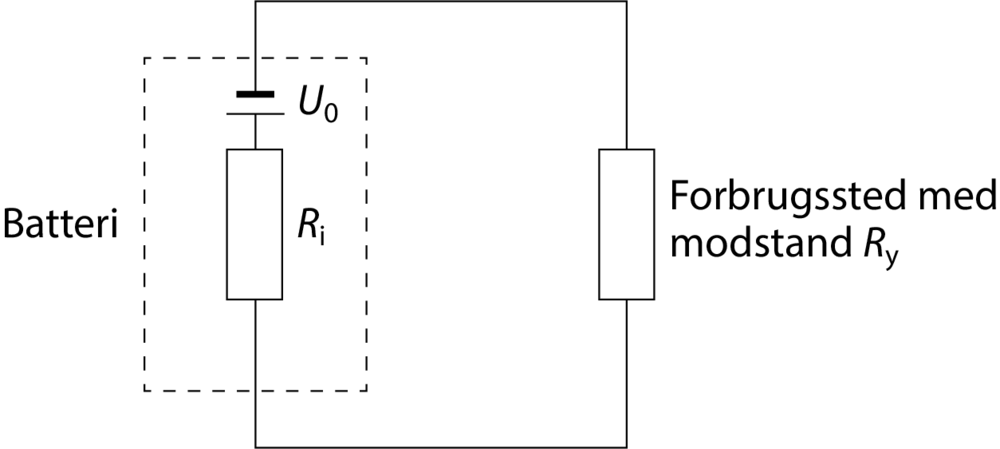
\includegraphics[width=0.6\linewidth]{./img/forsoeg_3.png}
\caption{\label{forsoeg_3}En model for en spændingskilde bestående af en superspændingskilde i serie med en indre modstand, som så igen er i serie med en ydre modstand. Figuren er lånt fra \url{https://orbithtxb.systime.dk/index.php?id=558}.}
\end{figure}

$$U_0 = R_i \cdot I + R_y \cdot I \,.$$

Dog er \(R_y \cdot I = U_p\), hvor \(U_p\) er \textbf{polspændingen}, og forrige ligning kan omskrives til:

\begin{align*}
    U_0 &= R_i \cdot I + U_p \iff \\
    U_0 - R_i \cdot I &= U_p \iff \\
    U_p &= - R_i \cdot I + U_0 \,.
\end{align*}

Hvis det sidste udtryk sammenlignes med ligningen for en ret linje

$$y = a \cdot x + b \,,$$

kan det ses, at \(U_p\) svarer til \(y\), \(-R_i\) svarer til hældningstallet \(a\), \(I\) svarer til \(x\) og \(U_0\) svarer til skæringen med y-aksen. Dette kan også ses grafisk på figur \ref{forsoeg_3_2}, hvor sammenhængen er indtegnet i et (\(I\), \(U_p\))-koordinatsystem.

\begin{figure}[htbp]
\centering
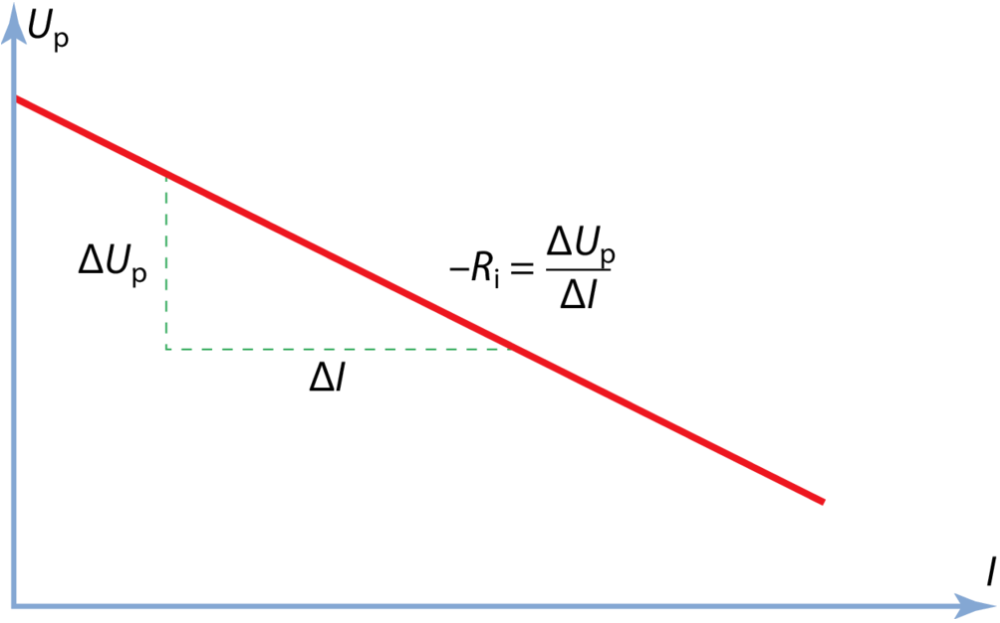
\includegraphics[width=0.6\linewidth]{./img/forsoeg_3_2.png}
\caption{\label{forsoeg_3_2}Den matematiske sammenhæng mellem polspændingen som funktion af strømstyrken. Figuren er lånt fra \url{https://orbithtxb.systime.dk/index.php?id=558}.}
\end{figure}

Som det ses, vil polspændingen falde som funktion af strømstyrken.
Det er præcis denne sammenhæng, der skal undersøges i dette eksperiment.

\subsection{Udstyr}
\label{sec:org97971dc}

Følgende udstyr skal anvendes til eksperimentet:

\begin{itemize}[noitemsep]
\item 1 amperemeter
\item 1 multimeter indstillet som voltmeter
\item 1 dekaderesitor (en variabel modstand)
\item Diverse nye og gamle 9V-batterier
\item Diverser ledninger til at opbygge kredsløbet med
\end{itemize}

\subsection{Fremgangsmåde}
\label{sec:org178b549}

Følg skridtene nævnt her:

\begin{figure}[htbp]
\centering
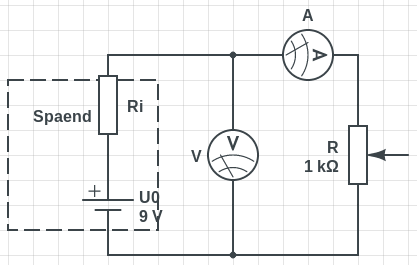
\includegraphics[width=0.6\linewidth]{./img/forsoeg_3_3.png}
\caption{\label{forsoeg_3_3}Det ønskede kredsløb til bestemmelse af den indre modstand etc. i et batteri.}
\end{figure}

\begin{enumerate}[noitemsep]
\item Opstil et kredsløb som ligner det på figur \ref{forsoeg_3_3}. Den stiplede boks repræsenterer et 9V-batteri.
\item Sørg for at dekaderesistoren er indstillet til høje værdier til at begynde med. Ellers tappes batterierne alt for hurtigt for energi.
\item Ændre på dekaderesistorens modstand og notér sammenhørende værdier af \(U_p\) og \(I\). Der skal opsamles mindst 10 målinger, gerne jævnt fordelt mellem tomgang (meget høj modstand) og kortsluttet tilstand (ingen modstand). \textbf{\textbf{I må dog ikke kortslutte batterierne}}.
\item Plot de opsamlede datapunkter i et (\(I\), \(U_p\))-koordinatsystem. Dette kan gøres i et regneark eller ved hjælp af geogebra.
\item \textbf{Fit} en ret linje til de plottede datapunkter, og aflæs/beregn, hvad henholdsvis hvilespændingen, kortslutningsstrømmen og den mindre modstand af batteriet er.
\end{enumerate}
\end{document}
